\documentclass[a4paper,10pt,ngerman]{scrartcl}
\usepackage{babel}
\usepackage[T1]{fontenc}
\usepackage[utf8x]{inputenc}
\usepackage[a4paper,margin=2.5cm,footskip=0.5cm]{geometry}

\newcommand{\Aufgabe}{Seminararbeit}
\newcommand{\TeilnahmeId}{76626}                 
\newcommand{\Name}{Quirin Klemm}            


% Kopf- und Fußzeilen
\usepackage{scrlayer-scrpage, lastpage}
\setkomafont{pageheadfoot}{\large\textrm}
\lohead{\Aufgabe}
\cfoot*{\thepage{}/\pageref{LastPage}}

% Position des Titels
\usepackage{titling}
\setlength{\droptitle}{-1.0cm}

\usepackage{float}


% Für mathematische Befehle und Symbole
\usepackage{amsmath}
\usepackage{amssymb}

% Für Bilder
\usepackage{graphicx}
\usepackage{fontspec}

\usepackage[hidelinks]{hyperref}

% Für Algorithmen
\usepackage{algpseudocode}

% Für Quelltext
\usepackage{listings}
\usepackage{color}
\definecolor{mygreen}{rgb}{0,0.6,0}
\definecolor{mygray}{rgb}{0.5,0.5,0.5}
\definecolor{mymauve}{rgb}{0.58,0,0.82}
\lstset{
  keywordstyle=\color{blue},commentstyle=\color{mygreen},
  stringstyle=\color{mymauve},rulecolor=\color{black},
  basicstyle=\footnotesize\ttfamily,numberstyle=\tiny\color{mygray},
  captionpos=b, % sets the caption-position to bottom
  keepspaces=true, % keeps spaces in text
  numbers=left, numbersep=5pt, showspaces=false,showstringspaces=true,
  showtabs=false, stepnumber=2, tabsize=2, title=\lstname
}

% Diese beiden Pakete müssen zuletzt geladen werden
%\usepackage{hyperref} % Anklickbare Links im Dokument
\usepackage{cleveref}

% Daten für die Titelseite
\title{\textbf{\Huge\Aufgabe}}
\author{\LARGE Teilnahme-ID: \LARGE \TeilnahmeId \\\\
	    \LARGE Bearbeiter/-in dieser Aufgabe: \\ 
	    \LARGE \Name\\\\}
\date{\LARGE\today}

\begin{document}

\maketitle
\tableofcontents

\vspace{0.5cm}


\clearpage

\section{Einleitung}
Die vorliegende Arbeit ist meine Einreichung für die zweiten Runde des 43. Bundeswettbewerb Informatik (BwInf).
Der Wettbewerb wird von der BWINF gGmbH ausgerichtet und von dem Bundesministerium sowie den Kultusministerien unterstützt.
Er gliedert sich in drei Runden, die aufeinander aufbauen. In der erste Runde, die in Gruppenarbeit durchgeführt wird, stehen fünf kleine Aufgaben zur Auswahl, von denen drei bearbeitet werden müssen. 
Die zweiten Runde erfolgt in Einzelarbeit; hierbei sind von drei angebotenen Aufgaben zwei zu lösen. 
Zur Endrunde werden die besten 30 Teilnehmer eingeladen, die an einem Wochenende ihr Wissen in einem Gespräch beweisen. [7]\\
In der ersten Runde gingen insgesamt 1790 Einsendungen ein, von denen 950 Teilnehmende zur zweiten Runde zugelassen wurden. [8]
In der zweiten Runde wurden nur noch 250 Lösungen eingereicht, aus denen die 30 besten Teilnehmer für die Endrunde ausgewählt wurden. [9]
Jede Aufgabe beschreibt ein Problem, für welches anschließend ein Algorithmus entwickelt werden soll, mit dem sich dieses lösen lässt.
Zusätzlich werden Testfälle gegeben, anhand derer der Algorithmus überprüft werden kann.
Die erwarteten Ergebnisse der Testfälle werden jedoch nicht angegeben. 
Sie dienen auschließlich dazu, dass die Korrektoren die Richtigkeit und Genauigkeit des Algorithmuses beurteilen können.
Die ausgearbeitet Lösungen werden anschließend nach einem festgelegten Schema korrigiert und benotet. Pro Aufgabe können bis zu 20 Punkte erreicht werden, 
wobei gute Ausarbeitungen Zusatzpunkte geben können und unvollständige Bearbeitungen Punktabzüge nach sich ziehen. [5]\\
Ich erreichte insgesammt 38 Punkte, erhielt damit den 2. Preis und (gehörte damit zu den besten 60 Teilnehmer).\\
Meine Arbeit ist in zwei Teile aufgeteilt, beginnend mit Aufgabe 1, Schmucknachrichten, und dann Aufgabe 2, simultane Labyrinthe.
Beide Teile sind gleich aufgebaut und entsprechen in ihrer Struktur den Vorlagen des BwInf-Teams,
abgesehen von der zusätzlichen Einleitung und dem eingefügten Vergleich mit der Musterlösung.\\
Zuerst erkläre ich kurz die Aufgabestellung. 
Danach beschreibe ich meine theorietische Überlegung und zeige im Anschluss, wie ich sie praktisch umgesetzt habe.
Anschließend diskutiere ich meine Ergebnisse, ziehe ein Fazit und vergleiche schließlich meine Lösung mit der offiziellen Musterlösung.
\section{Aufgabe 1: Schmucknachrichten}
\subsection{Einleitung}
In dieser Aufgabe möchten Sybille und Pedram kurze Nachrichten, die aus verschiedenen Buchstaben bestehen, in Perlen-Codes für Ketten umwandeln.
Für jeden Buchstaben ist ein Codewort aus Perlen zu finden, wobei insgesamt ein präfixfreier Code entstehen muss.
Dabei soll die Gesamtlänge der codierten Nachricht möglichst gering sein.
Daher wird ein präfixfreier Code gesucht, bei dem häufig vorkommende Buchstaben kurze Codewörter erhalten, während seltenere Buchstaben längere Codewörter zugewiesen bekommen. 
"Ein Code C heißt Prafix-Code (irreduzibler Code), wenn kein Codewort aus C Prafix eines anderen Codeworts von C ist." [10]
Dadurch lässt sich jede Nachricht eindeutig codieren und wieder decodieren.
Ein Code mit den Codewörtern {a, ba, bb} ist präfixfrei, da kein Codewort der Anfang eines anderen ist.
Im Gegensatz dazu ist der Code {a, ab, bb} nicht präfixfrei ist, weil "a" der Präfix von "ab" ist.
Zusätzlich wird in dieser Aufgabe zwischen zwei Varrianten unterschieden:
In der ersten Teilaufgabe haben alle Perlen denselben Durchmesser, 
während in der zweiten Teilaufgabe die Perlen unterschiedliche Durchmesser besitzen.\\
Ich bearbeite zuerst die Aufgabe, mit den gleichen Durchmessern, und anschließen mit unterschiedlichen Durchmessern. (vgl.)[5]
\subsection{Lösungsidee}
\subsubsection{Perlen mit gleichen Durchmessern}
In meiner Arbeit gilt die Annahme, solange alle Perlen im Durchmesser gleich sind:
\begin{equation}
  \label{Kosten eines Buchstaben}
  c_i = p_i \cdot n_i
\end{equation}

\begin{equation}
  \label{equation:simple_kostenberechnung}
  l = \sum_i c_i
\end{equation}
- $c_i$ die Kosten des Buchstaben $i$ \\
- \( p_i \) die Häufigkeit des Buchstabens \( i \) in der Nachricht   \\
- \( n_i \) die Länge des Codewortes für den Buchstaben \( i \) (Anzahl der Perlen)  \\
- \( l \) die Länge der codierten Nachricht \\ 
\\
Die Gesamtlänge der Nachricht entspricht der Summe aller Kosten jedes einzelnen Buchstabens.\\
Um einen präfixfreien Code zu erzeugen, wird meist ein Baum benutzt. 
Jeder präfixfreie Code kann in einem Baum dargestellt werden und jeder Baum kann einen präfixfreien Code darstellen. [10]
Durch diesen sicher gestellt werden, dass kein Codewort der Anfang eines anderen Codeworts ist
Den gleichen Ansatz 
(genauer erklären warum bäume. hab ich mich selber überlegt. und literatur hab es auch dannach wieder gefunden).
Da durch diesen sicher gestellt werden kann, dass kein Codewort der Anfang eines anderen Codeworts ist.
\\
In dieser Arbeit ist ein Baum definiert als Blatt des Baums ein Codewort und jede Kante zum Blatt ein Teil des Codeworts. (todo: rewrite)
Der Baum hat mindestens so viele Blätter wie es verschiedene Buchstaben gibt.
Jeder innere Knoten hat dabei maximal so viele Kinder, wie es verschiedene Perlen gibt. 
Die Ebene des Blatts entspricht der Länge des Codeworts, also $n$.

\begin{figure}[h]
  \centering
  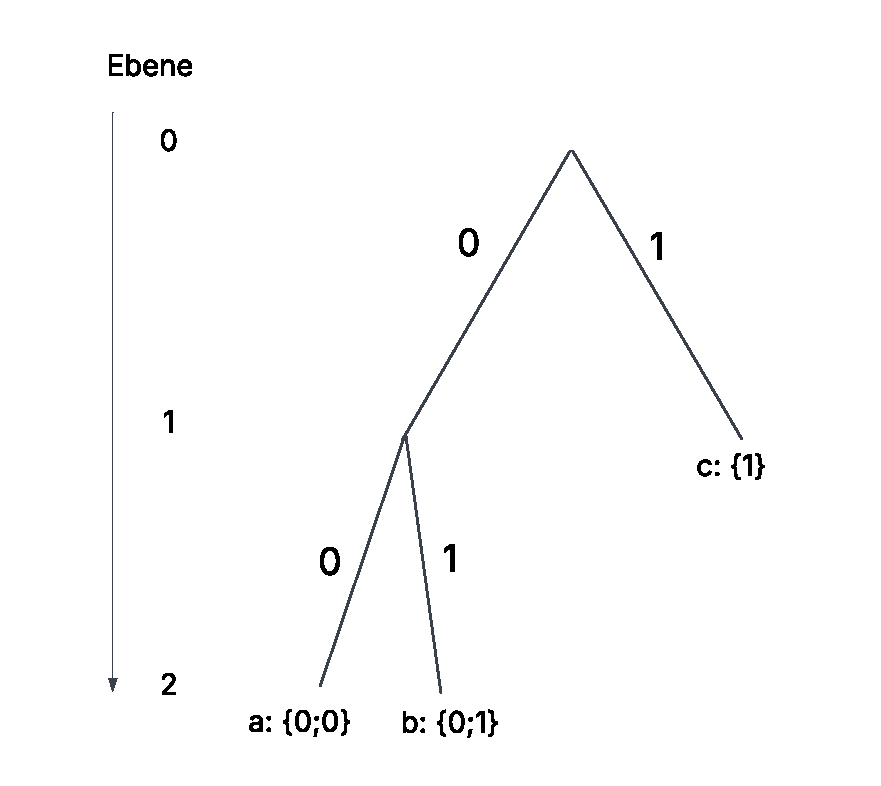
\includegraphics[width=0.6\textwidth]{Schmucknachrichten/pdf_src/simple_tree.pdf}
  \caption{simple tree}
  \label{fig:simple tree}
\end{figure}

Um einen möglichst kleinen präfixfreien Code zu erstellen, muss der Buchstabe, der am häufigsten vorkommt, ganz oben eingeordnet werden und die nächsten Buchstaben dann in absteigender Reihenfolge. 
In Abbildung \ref{fig:simple tree} hätte c die höchste Häufigkeit und danach kommt a und b. 
Ob der Buchstabe a oder b die höhere Häufigkeit besitzt, ist nicht relevant, da beide auf der untersten Ebene sind.\\
\\
Daher ergibt sich $p_1 \geq p_2 \geq p_3 ... \geq p_i$ und $n_1 \leq n_2 \leq n_3 ... \leq n_i$\\
\\
Zu finden ist also ein Baum, der basierend auf den Häufigkeiten der Buchstaben, seine Blätter so auf seine Ebenen verteilt, dass die Länge der codierten Nachricht (Gleichung \eqref{equation:simple_kostenberechnung}) möglichst gering ist. 
Jeder innere Knoten muss dabei mindestens zwei Kinder haben, da ein innerer Knoten mit nur einem Kind die Äste des Baums verlängert (höheres $n$) ohne einen Vorteile zu bringen.\\

Zu Beginn des Algorithmus wird ein balancierter Baum erstellt, der so viele Blätter wie Buchstaben hat (Abbildung \ref{fig:balancierter_Baum}). 
Jedes Blatt wird von links nach rechts in aufsteigender Reihenfolge der Häufigkeit, mit einem Buchstaben belegt, und die Gesamtkosten des Baums werden gemäß der Formel \eqref{equation:simple_kostenberechnung} berechnet. 
Dabei ergeben sich deutlich höhere Kosten für die rechten Buchstaben im Baum im Vergleich zu den linken, da alle Blätter auf derselben Ebene sind, jedoch die Häufigkeit der Buchstaben auf der rechten Seite größer ist.
Um dies auszugleichen, wird der Buchstabe mit den höchsten Kosten eine Ebene nach oben verschoben,
indem der Elternknoten des Blattes selber zum Blatt wird und alle Kinder verliert.
Dadurch verliert der Baum aber zu viele Kinder, weshalb er erweitert werden muss.
Für die Erweiterung untersucht der Algorithmus, an welche Knoten neue Blätter angehängt werden können. Er überprüft die Blätter nach ihrer Ebene, d.h. nach ihrem Wert für $n$,
und fügt das mit dem kleinsten Wert hinzu.
Das nach oben verschobenene Blatt erhält den Zusatz $protected$. 
Das verhindert, dass es selbst weitere Kinder bekommen kann.
Nach jeder Iteration werden den Blättern wie zu Beginn von links nach rechts Buchstaben aufsteigend hinzugefügt.
Das stellt sicher, dass immer die äußerst linken Blätter (d.h. die mit dem höchsten $n$-Wert), die Buchstaben mit den geringsten Häufigkeiten kriegen und rechts die höchsten.
Dadurch wird ein Zyklus vermieden, bei dem ein Blatt zunächst nach oben verschoben und anschließend wieder nach unten erweitert würde.\\
Das Verschieben der Blätter nach oben, sowie das Neueinfügen der Blätter unten, gilt als ein Optimierungsschritt,
welcher im Optimierungsprozess wiederholt wird. (Abbildung \ref{fig:trans_2})
Dieser Vorgang wird so lange fortgesetzt, bis keine neuen Blätter mehr eingefügt werden können, da alle Blätter als $protected$ gelten (Abbildung \ref{fig:baum_fertig}) - also keine weiteren Optimierungen mehr möglich sind.
Das ist der Fall kurz vor einem maximal ausgearteten Baum.
Der Algorithmus geht also von einem Maximum (maximal ausbalanciert) zum anderen Maximum (maximal ausgeartet).
Am Ende wird der Baum mit den geringsten Gesamtkosten ausgegeben.

\begin{figure}[h]
  \centering
  \begin{minipage}{0.49\textwidth}
    \centering
    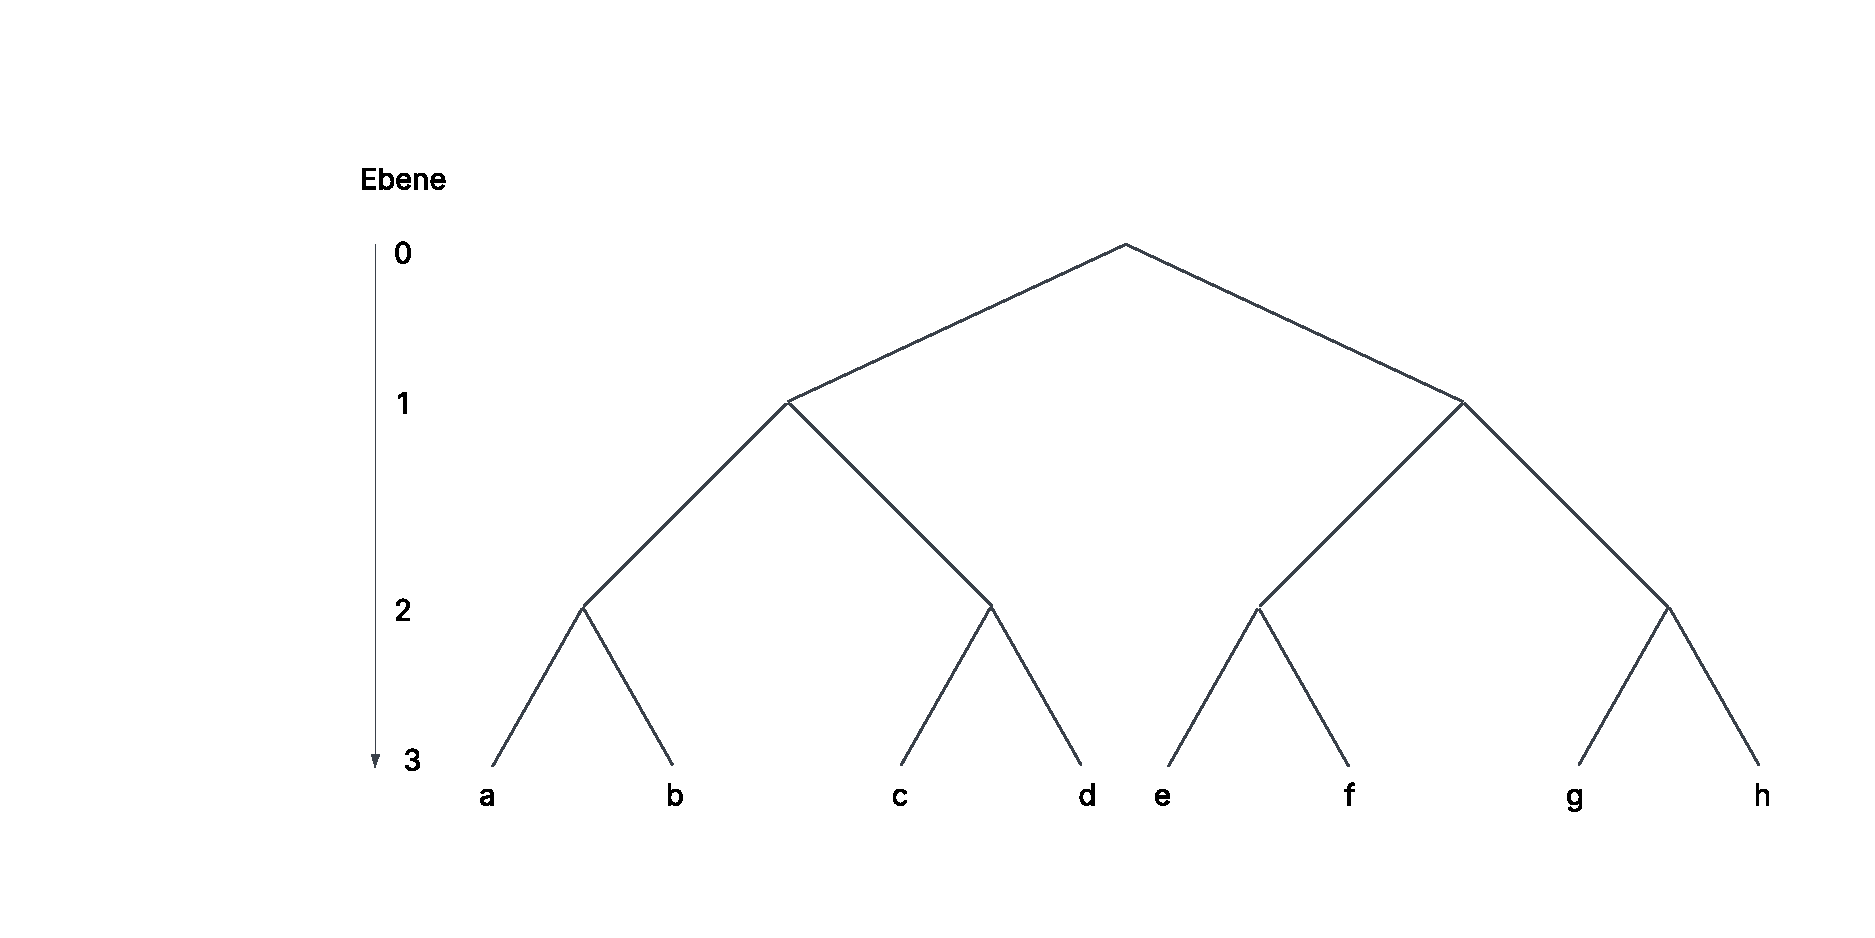
\includegraphics[width=\textwidth]{Schmucknachrichten/pdf_src/trans_1.pdf}
    \caption{Balancierter Baum}
    \label{fig:balancierter_Baum}
  \end{minipage}
  \hfill
  \begin{minipage}{0.49\textwidth}
    \centering
    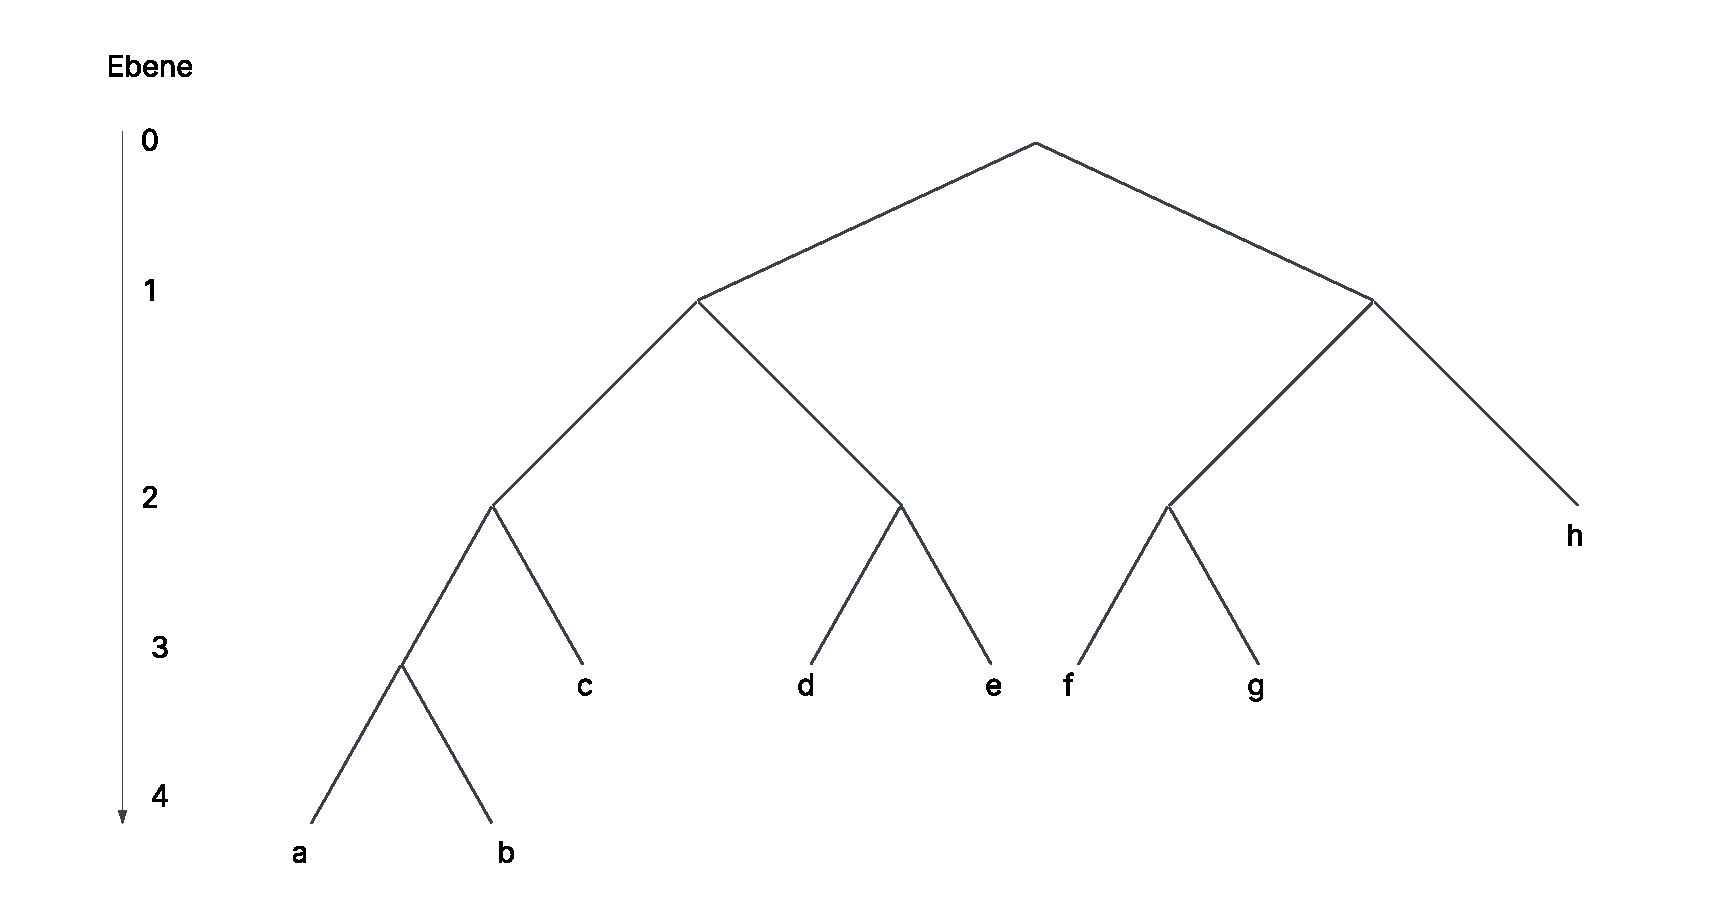
\includegraphics[width=\textwidth]{Schmucknachrichten/pdf_src/trans_2.pdf}
    \caption{Transformation 1}
    \label{fig:trans_1}
  \end{minipage}
\end{figure}

\begin{figure}[h]
  \centering
  \begin{minipage}{0.5\textwidth}
    \centering
    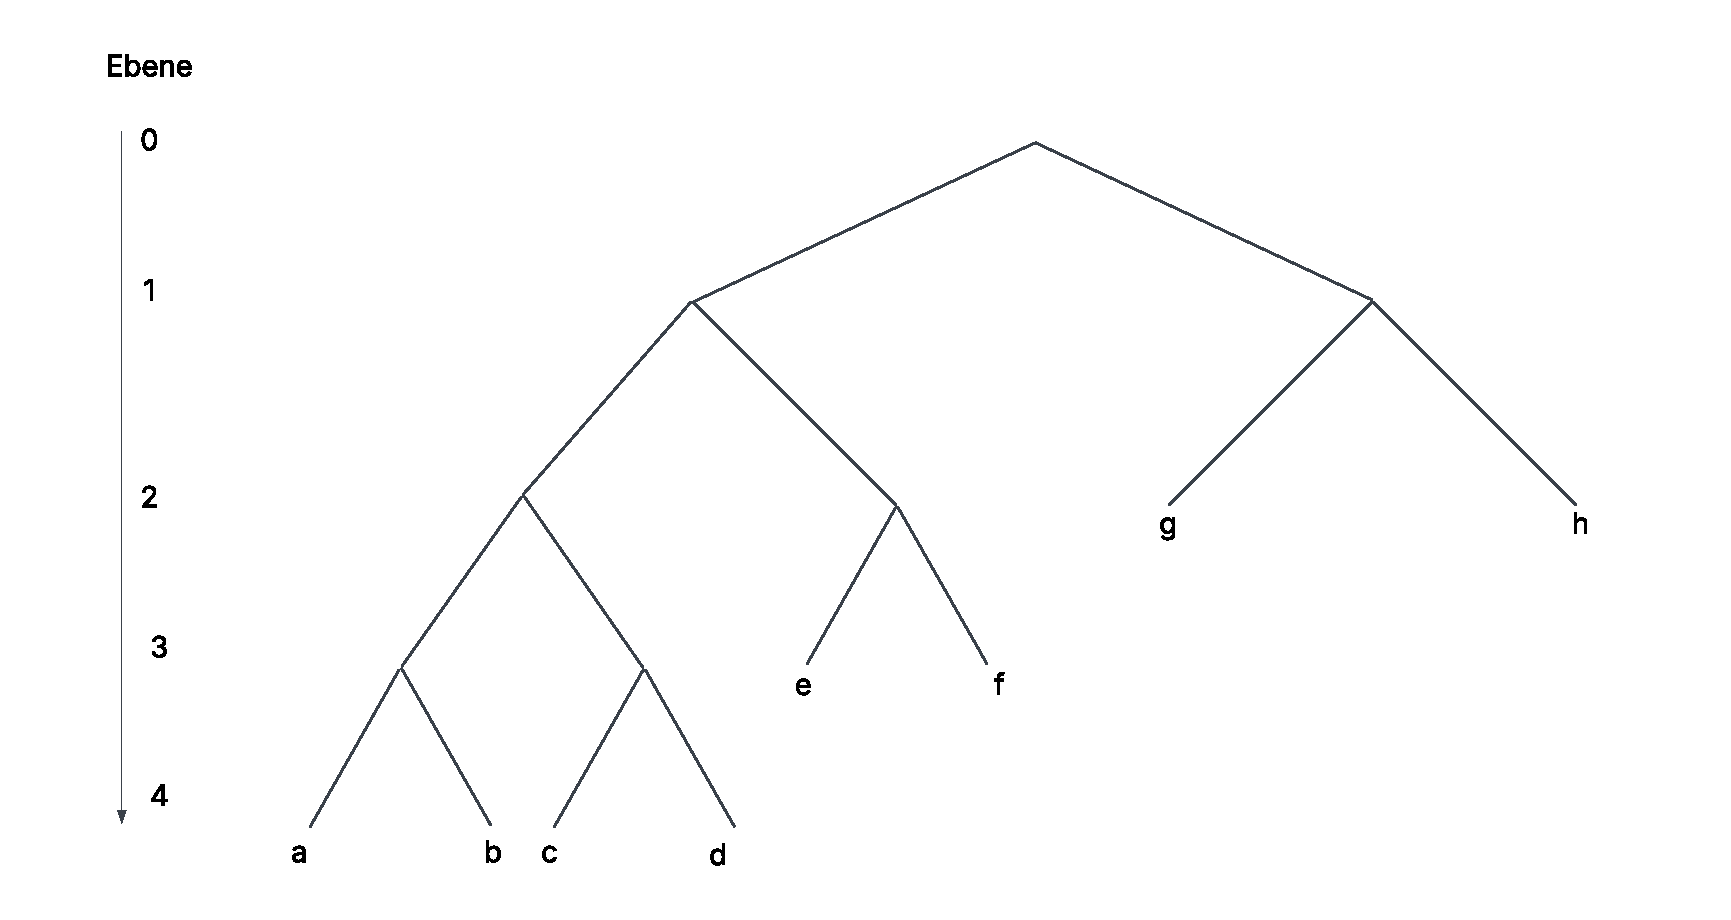
\includegraphics[width=\textwidth]{Schmucknachrichten/pdf_src/trans_3.pdf}
    \caption{Transformation 2}
    \label{fig:trans_2}
  \end{minipage}
  \hfill
  \begin{minipage}{0.3\textwidth}
    \centering
    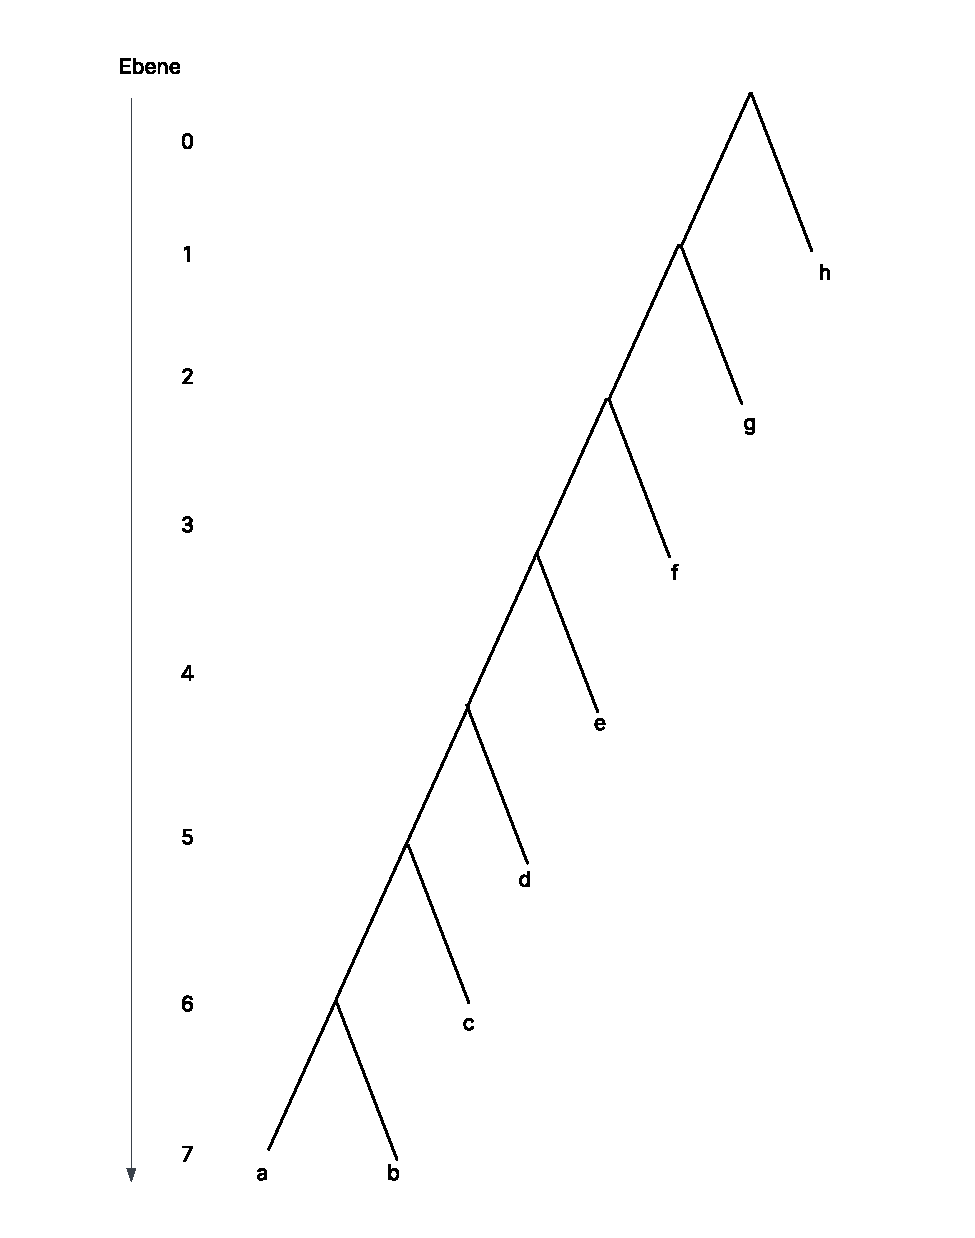
\includegraphics[width=\textwidth]{Schmucknachrichten/pdf_src/trans_4.pdf}
    \caption{Ausgearteter Baum}
    \label{fig:baum_fertig}
  \end{minipage}
\end{figure}

\subsubsection{Perlen mit unterschiedlichen Durchmessern}
Das Problem bei unterschiedlichen Perlendurchmessern besteht darin, dass Blätter auf derselben Ebene unterschiedliche Kosten für die Gesamtlänge der Nachricht haben können.
Daher sind die Kosten nicht mehr der Wert der Ebene und damit die Anzahl an Perlen.
Das hat zur Folge, dass die Gleichung \eqref{Kosten eines Buchstaben} nicht mehr stimmt.
Stattdessen muss der Durchmesser jeder Perle im Codewort einzeln angeschaut werden. Daher ergibt sich

 \begin{equation}
  \label{Neue Kosten eines Buchstaben}
  c_i = p_i \cdot \sum_n cp_n
 \end{equation}


 - $cp_n$ die Kosten/Durchmesser der Perle $n$\\

 Stellt man nun Bäume nicht nach ihrer Ebene, sondern nach ihren Kosten dar, erhält man einen \textit{lopsided tree} [1].

 \begin{figure}[h]
  \centering
  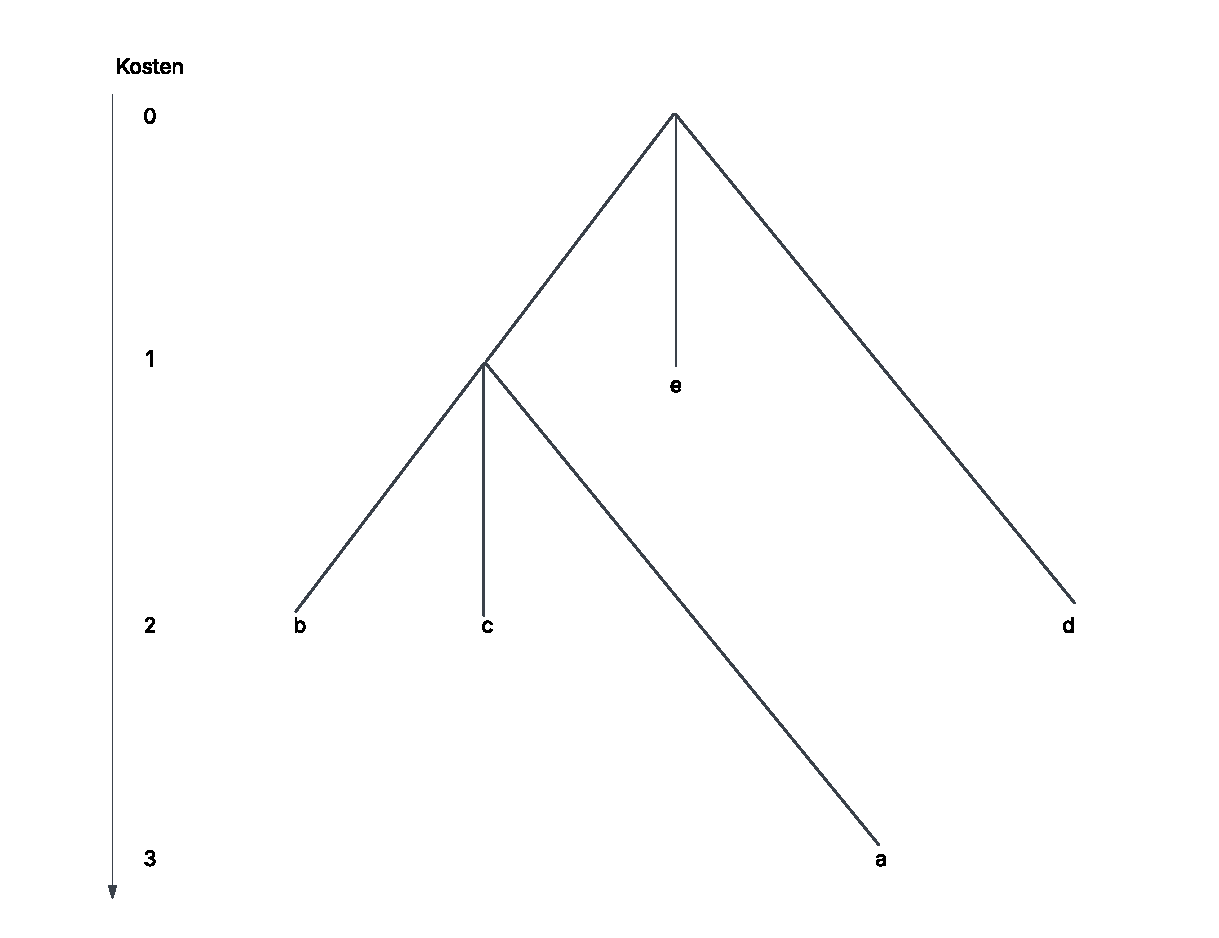
\includegraphics[width=0.6\textwidth]{Schmucknachrichten/pdf_src/lopsided_tree.pdf}
  \caption{lopsided tree: Perlendurchmesser: (1; 1; 2) }
  \label{fig:lopsided tree}
\end{figure}
Auch hier gilt: Jeder innere Knoten muss mindestens zwei Kinder haben. 
Bei dieser Art von Bäumen hat jedoch nicht der äußerst rechte Knoten die geringsten Kosten, sondern der oberste.
Der Algorithmus bleibt unverändert: Zunächst wird ein Baum erstellt, in dem alle Blätter ungefähr die gleichen Kosten haben. 
Anschließend wird der Buchstabe mit den höchsten Kosten nach oben verschoben, während der Baum unten erweitert wird.
Dies geschieht solange, bis kein Blatt mehr eingefügt werden kann und der beste Baum wird ausgegeben.
\\
Wenn die Durchmesser alle gleich groß sind, gilt: 
\begin{equation}
 p_i \cdot n_i = p_i \cdot \sum_n cp_n
\end{equation} 
daher kann der zweite Algorithmus sowohl für gleiche als auch unterschiedliche Durchmesser benutzt werden.


\subsection{Umsetzung}
(Die Lösung wurde in Python3 geschrieben. Die Eingabetexte werden eingelesen, anhang) Die Durchmesser der Perlen werden in einer Liste gespeichert und der Text in einem string.
Aus dem Text werden anschließend zwei Listen erstellt:
Die erste enthält die Häufigkeiten der Buchstaben in absteigender Reihenfolge.
Die zweite enthält die Buchstaben entsprechend dieser Reihenfolge. (todo: rewrite)
Sie sehen für Beispielaufgabe $schmuck0$ so aus:\\
1. [6, 3, 3, 2, 2, 1]\\
2. ['d', 'a', 's', 'f', 'g', 'h']\\
Um später den Buchstaben die Häufigkeit wieder richtig zuzuordnen.

\begin{figure}[h]
  \centering
  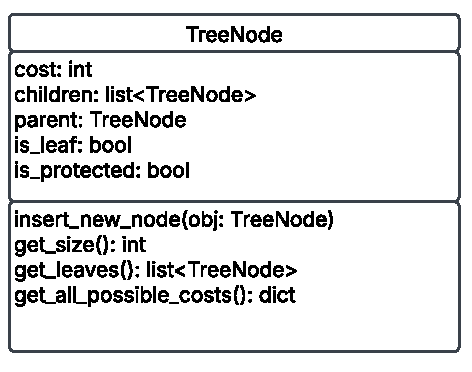
\includegraphics[width=0.6\textwidth]{Schmucknachrichten/pdf_src/klassen_diagramm.pdf}
  \caption{TreeNode Klasse}
  \label{fig:klassn_daigramm}
\end{figure}

\subsubsection{Erstellung des Baums}
Zu Beginn wird ein blancierter Baum über die Methode $create\_tree()$ erstellt.
\vspace{2em}

\begin{lstlisting}[caption={Methode \texttt{create\_tree}}, label={lst:create_tree}]
  def create_tree(root: TreeNode) -> TreeNode:
\end{lstlisting}
Die Methode $create\_tree$ bekommt jedes potenziell neue Blatt im Baum über den Aufruf $get\_all\_possible\_costs()$ (todo: rewrite)
und das Blatt mit den geringsten Kosten wird dem Baum über den Aufruf $insert\_new\_node(obj)$ hinzugefügt.
Falls der Elternknoten des neuen Blatts selbest noch ein Blatt ist, entsprechen die Kosten des neuen Blatts den kombinierten Kosten für die ersten beiden Blätter.
Das liegt daran, dass jeder innere Knoten mindesten zwei Kinder haben muss – daher stellen diese Kosten die effektiv neu entstehenden Kosten für den Baum dar.
Das geschieht solange, bis der Baum genau so viele Blätter hat, wie es Buchstaben gibt. Seine Anzahl an Blättern erhält er über die Methode $get\_size()$.

\vspace{2em}

\begin{lstlisting}[caption={Methode \texttt{get\_all\_possible\_costs}}, label={lst:get_all_pssible_costs}]
  def get_all_possible_costs(self) -> dict:
\end{lstlisting}
Die Methode $get\_all\_possible\_costs$ prüft, ob das TreeNode-Objekt noch weitere Kinder aufnehmen kann und nicht protected ist.
Falls ja, fügt es sich selbst sowie die Kosten des potenziellen neuen Kindes einem Dictionary hinzu.
Anschließend wird die Methode rekursiv für alle bestehenden Kinder aufgerufen, so dass auch deren mögliche Erweiterungen im Dictionary erfasst werden.\\
\\
\vspace{2em} 
\begin{lstlisting}[caption={Methode \texttt{insert\_new\_node}}, label={lst:insert_new_node}]
  def insert_new_node(self, obj: TreeNode):
\end{lstlisting}
Die Methode $insert\_new\_node$ prüft, ob das aktuelle Objekt selbst das gesuchte TreeNode Objekt ist. Falls ja, fügt es ein neues Kind hinzu. 
Wenn vorher noch keine Kinder vorhanden sind, werden zwei Kinder hinzugefügt.
Ansonsten wird die Methode rekursiv auf alle bestehenden Kinder angewandt.\\
\\

\vspace{2em} 
\begin{lstlisting}[caption={Methode \texttt{get\_size}}, label={lst:get_size}]
  def get_size(self) -> int:
\end{lstlisting}
\vspace{0.5em}
Die Methode $get\_size$ gibt den Wert 1 zurück, falls das Objekt ein Blatt ist. Ansonsten wird die Methode rekursiv bei den Kinder aufgerufen und die Summe zurückgegeben.

\subsubsection{Verbesserung des Baums}
Sobald ein balancierter Baum erstellt wurde, muss dieser optimiert werden. Dies geschieht über die Methode $find\_best\_tree$.
\vspace{2em}
\begin{lstlisting}[caption={Methode \texttt{find\_best\_tree}}, label={lst:find_best_tree}]
  def find_best_tree(root: TreeNode) -> TreeNode:
\end{lstlisting}
Die Methode $find\_best\_tree$ versucht, den übergebenen Baum so lang zu optimieren, bis alle Blätter als $protected$ markiert sind und keine Blätter mehr hinzugefügt werden können.
Dazu wird der Optimierungsschritt über den Aufruf $improve\_tree(root)$ wiederholt und jeweils mit der Methode $calculate\_tree(root)$ die neuen Kosten des Baums berechnet.
Sind die neuen Kosten ein neues Minimum wird der aktuelle Baum als bester Zwischenstand gespeichert.
Können keine neuen Blätter dem Baum hinzugefügt werden und es tritt ein Fehler auf, wird der bis dahin beste gefundene Baum zurückgegeben.\\
\\
\vspace{2em}
\begin{lstlisting}[caption={Methode \texttt{imporve\_tree}}, label={lst:imporve_tree}]
  def improve_tree(root: TreeNode) -> TreeNode:
\end{lstlisting}
Zu Beginn holt sich die Methode $improve\_tree$ alle Blätter im Baum über den Aufruf $get\_leaves()$.
Diese Liste wird dann aufsteigend sortiert und die Kosten für jedes Element können mit der Gleichung \eqref{Neue Kosten eines Buchstaben} berechnet werden.
Der Elternknoten des Blatts mit den höchsten Kosten wird daraufhin selbst zu einem Blatt. Dafür werden die Attribute des Elternknoten
\begin{lstlisting}
  is_leaf = True
  is_protected = True
  children = []
\end{lstlisting}
\vspace{-1.5em}
gesetzt. Um die fehlenden Blätter wieder hinzuzufügen wird noch die Methde \ref{lst:create_tree}  ($create\_tree$) aufgerufen.\\
\\\\
\begin{lstlisting}[caption={Methode \texttt{calculate\_tree}}, label={lst:calculate_tree}]
  def calculate_tree(root: TreeNode) -> TreeNode:
\end{lstlisting}
Die Methode $calculate\_tree$ berechnet die gesamt Kosten des Baums. Dafür holt sie sich auch über den Aufruf $get\_leaves()$ alle Blätter im Baum.
Die Liste an Blättern wird dann nach den Kosten aufsteigend sortiert und jedes Element wird wie in der Gleichung \eqref{Neue Kosten eines Buchstaben} berechnet und zusammenaddiert.




\subsection{Laufzeit und Diskussion}
\begin{figure}[h]
  \centering
  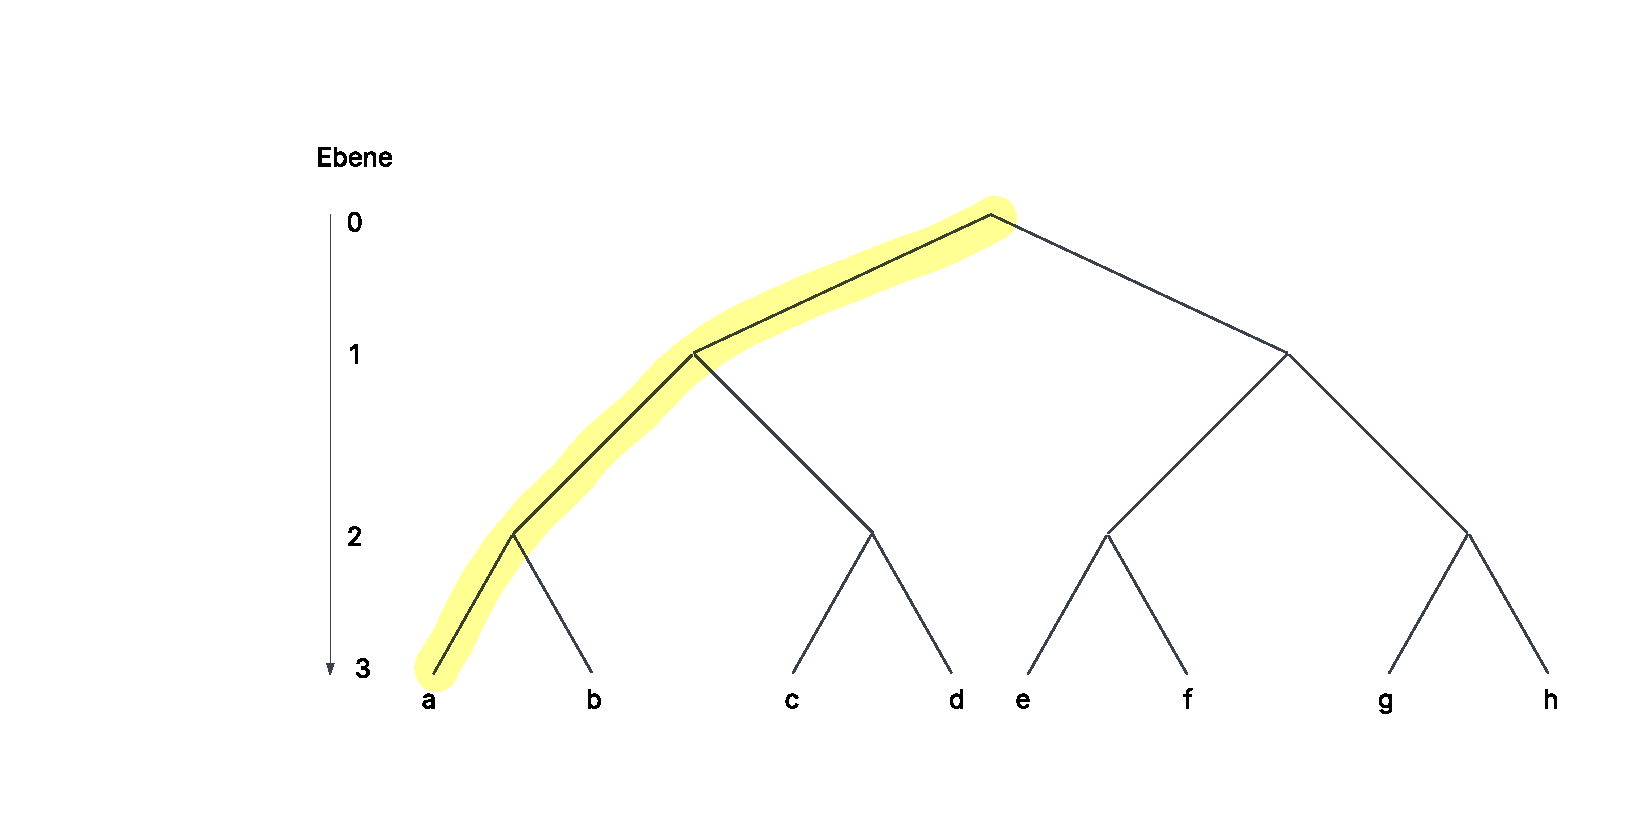
\includegraphics[width=0.6\textwidth]{Schmucknachrichten/pdf_src/trans_makiert.pdf}
  \caption{Balancierter Baum, Markierung der richtigen Knoten}
  \label{fig:makiert_baum}
\end{figure}



\subsubsection{Analyse des Algorithmus}
Der Algorithmus endet, wenn keine Knoten mehr eingefügt werden können.
Dies ist spätestens gegeben, wenn der Baum maximal ausgeartet ist (Abbildung \ref{fig:baum_fertig}).
Allgemein kann jeder Knoten maximal $r-1$ Mal verschoben werden, bis er komplett auf der linken Seite ist. Dabei ist $r$ die Anzahl an verschiedenen Perlen.
Daraus folgt, dass die maximale Anzahl an Iterationen  
\begin{equation}
  I < (r-1)\cdot\text{Anzahl falscher Knoten}
\end{equation}
ist, bis zum maximal ausgearteten Baum.
Falsche Knoten sind dabei innere Knoten, die beim ausbalancierten Baum noch nicht auf der richtigen Stelle sind, also alle bis auf die äußerst linken Knoten. (Abbildung \ref{fig:makiert_baum})

Generell gilt, um die maximale Anzahl an inneren Knoten zu erhalten, sollte jeder Knoten möglichst wenig Kinder besitzen.
Wie zuvor festgelegt, hat jeder innere Knoten mindestens zwei Kinder. 
Daraus folgt, dass die maximale Anzahl an inneren Knoten erreicht wird, wenn der Baum ein Binärbaum ist und kann durch
\begin{equation}
  \text{innere Knoten} = w - 1
\end{equation}
berechnet werden.
Dabei ist $w$ die Anzahl an Blättern/Codewörter.
Auf jeder Ebene existiert ein richtiger innere Knoten, deren Anzahl minimal mit 
\begin{equation}
  \text{richtige innere Knoten} = \log_{r-1}{w}
\end{equation}
abgeschäzt werden kann.\\
Daher ergibt sich
\begin{equation}
  I < (r-1)\cdot(w-1-\log_{r-1}{w})
\end{equation}
Dies bedeuted eine Laufzeit von $O(r\cdot w)$.


\begin{figure}[H]
  \centering
  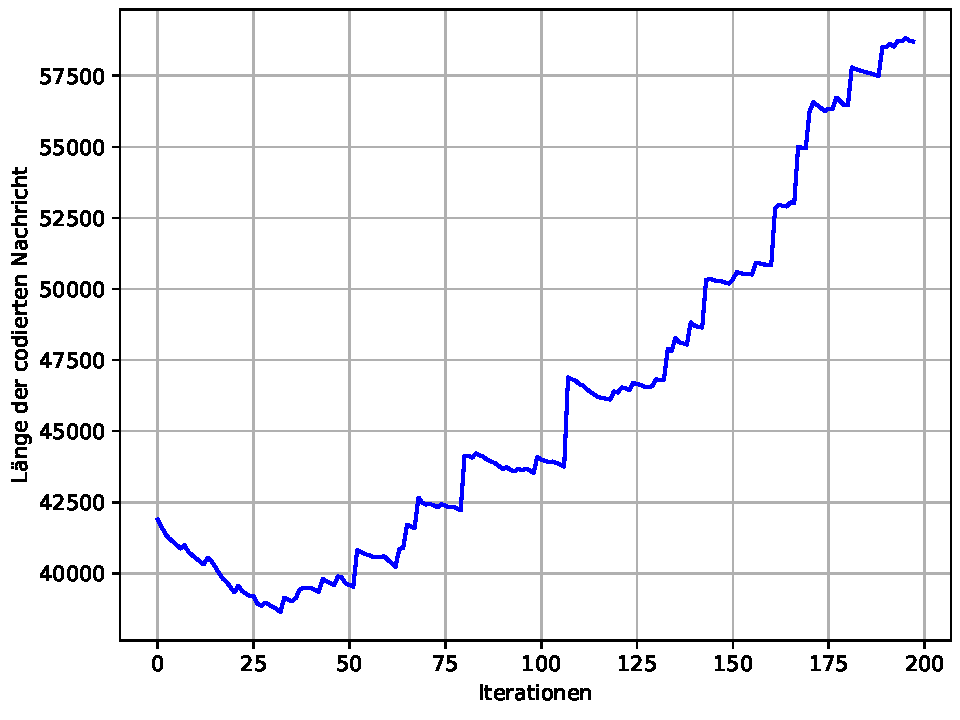
\includegraphics[width=0.6\textwidth]{Schmucknachrichten/pdf_src/genauigkeit_iterationen.pdf}
  \caption{Länge der codierten Nachricht über mehrere Iterationen}
  \label{fig:iteration_tree}
\end{figure}
Abbildung \ref{fig:iteration_tree} zeigt wie die Länge der codierten Nachricht der Beispielaufgabe $schmuck9$ sich über die Iterationen hinweg verändert.
Das Minimum wird bereits in der ersten Hälfte der Iterationen erreicht.
\subsubsection{Stand der Forschung}
Die vorliegende Fragestellung ist seit den 60iger-Jahren in der theorietischen Informatik bekannt. 
Dabei lieferte Huffman eine Lösung für den Spezialfall, von zwei Quellsymbolen. [3]
\\
\\
Für unseren Fall von mehr als zwei Quellsymbolen mit unterschiedlichen Kosten, 
entwickelte bereits Richard Karp 1961 [4] eine Lösung. Diese wurde 1998 von Mordecai J. Golin und Günter Rote verbessert und ist bis heute das schnellste Verfahren, um auf eine exakte Lösung zu kommen.\\
"The minimum-cost prefix-free code for n words can be computed in $O(n^{C+2})$ time and $O(n^{C+1})$ space, if the costs of the letters are integers between 1 and C."\\
Für die Beispielaufgabe $schmuck5.txt$ hat der Algorithmus eine Laufzeit $34^8$(n=34; C=6) Iterationen. 
Diese Art von Algorithmus kann wegen seiner langen Laufzeit nicht für die vorgegebenen Beispielaufgabe verwendet werden. [1]
\\
\\
Um eine polynominelle Laufzeit zu erreichen, entwickelten Mordecai J. Golin, Claire Mathieu und Neal E. Young 2012 ein Approximationsverfahen.\\
Dieser Algorithmus basiert auf dem PTAS-Verfahren, wobei zuerst ein präfixfreier Code bis zur einer bestimmten Tiefe $\tau$ erstellt wird und dann die restlichen Codewörter durch ein Rundungsverfahren ergänzt werden.
Dabei ist es zentral, dass die Wahrscheinlichkeitsverteilung der zu kodierenden Codewörter möglichst in großen Gruppen mit gleich großer Wahrscheinlichkeit eingeordnet werden können.
In den Beispielen, vor allem in Beispiel 9 ist dies nicht gegeben, weshalb das Bestimmen des Vorbaums über $9^{24}$ Schritte benötigt.
Somit ist dieses Verfahren für die gewählten Beispiele ebenfalls nicht verwendbar. [2]

\subsubsection{Fazit}
Für die gegeben Fragestellung gibt es bislang weder ein Beweis, dass sie NP-schwer ist, als auch keinen Gegenbeweis, dass sie es nicht ist.
Aktuell bekannte Verfahren besitzen eine exponnentielle Laufzeit. [1]
Mein vorgestellter Algorithmus findet nicht die beste Lösung für das gegebene Problem. Er liefert jedoch in polynomieller Laufzeit eine gute Approximation
und ist daher eine gute Abwägung zwischen Laufzeit und Genauigkeit.
Somit wird nicht beantwortet, ob die Fragestellung NP-schwer ist.


\subsection{Vergleich zur Lösung}
In der Musterlösung werden drei Lösungen vorgeschlagen:\\
1. ein Greedy-Algorithmus bassierend auf Huffman\\
2. ein ILP-Ansatz nach Richard Karp und\\
3. die Erweiterung von Mordecai J. Golin und Günter Rote (vgl.) [6]\\
Alle drei Ansätze waren mir bei Abgabe meiner Arbeit bekannt (siehe Abschnitt 2.4.3). 
Trotzdem entschied ich mich dagegen eines dieser Verfahren zu implementieren, vorallem aufgrund derren hohen Laufzeit, 
und entwickelte stattdessen meine eigenes Verfahren.
Mein Algorithmus hat dabei eine durchschnittliche Abweichung von 1,27\% vom ideal Ergebnis, besitzt aber dafür eine sehr viel kürzere Laufzeit. 
(Todo: Hinweis auf die Lösungen)
Für mein gutes Ergebnis erhielt ich daher auch eine Pluspunkt.
Da ich außerdem zu allen Teilaspekten der Aufgabe Stellung nahm und keine Punkte abgezogen wurden, erreichte ich insgesamt 21 Punkte für diese Aufgabe.

\section{Aufgabe 2: Simultane Labyrinthe}
\subsection{Einleitung}
In dieser Aufgabe möchten drei Freunde, Anton, Bea und Chris, zwei Labyrinthe gleichzeitig durchlaufen.
Beide Labyrinth haben die selben rechteckigen Maße (n, m).
Zwei starteten jeweils in einem Labyrinth bei der Position (0, 0) und müssen das Ziel (n, m) erreichen, also von der linken oberen Ecke zur rechten unteren Ecke.
Ein dritter gibt jeweils beiden immer dieselbe nächste Schrittanweisung. 
Ist der nächste Schritt in einem Labyrinth durch eine Wand blockiert, bleibt die Person stehen.
Gesucht ist eine möglichst kurze Abfolge von Schritten, die beide Labyrinthe mit den selben Befehlen löst.
Bei dieser Aufgabe wird zusätzlich zwischen zwei Varianten unterschieden: 
in der ersten Teilaufgabe handelt es sich um Labyrinthe ohne Grube und in der zweiten Teilaufgabe um Labyrinth mit Grube.
Fällt ein Spieler in eine Grube, wird seine Position auf die Startposition (0, 0) zurückgesetzt.
Ich bearbeite zuerst die Variante ohne die Gruben und erweitere sie anschließend auf Labyrinthe mit Gruben. (vgl.) [5]
\subsection{Lösungsidee}
Zu Beginn wird für jedes Labyrinth eine Matrix erstellt (Abbildung \ref{fig:lybnmatrix}),
in der für jede Position ein Tuple aus einem Kostenwert und einer Richtung gespeichert wird. 
Die gespeicherte Richtung zeigt den optimalen Folgeschritt zum Ziel und ist dargestellt als
\begin{table}[h]
  \centering
  \begin{tabular}{|c|l|}
      \hline
      \textbf{Code} & \textbf{Richtung} \\
      \hline
      0 & Rechts \\
      1 & Links \\
      2 & Oben \\
      3 & Unten \\
      \hline
  \end{tabular}
  \caption{Codierung der Richtungen im Labyrinth}
  \label{tab:richtungscodierung}
\end{table}
\\
Der Kostenwert gibt an, wie viele Schritte bis zum Ziel benötigt werden.\\
Ein Labyrinth mit dazugehöriger Matrix könnte so aussehen:
\begin{figure}[H]
  \centering
  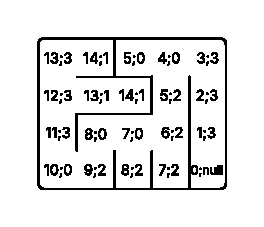
\includegraphics[width=0.4\textwidth]{Simultane Labyrinthe/pdf_src/cost_matrix.pdf}
  \caption{Labyrinth und Matrix}
  \label{fig:lybnmatrix}
\end{figure}

\subsubsection{Erstellung der Matrix}
Zu Beginn wird eine Matrix erstellt, deren Werte für alle Positionen zunächst leer sind.
Ausgehend vom Zielpunkt durchläuft der Algorithmus rekursiv alle erreichbaren Nachbarpositionen.
Für jeden Nachbarn wird in der Matrix ein Kostenwert eingetragen, der um eins höher ist als der Kostenwert des aktuellen Punkts, sowie die Richtung, aus der der Nachbar erreicht wurde.


\subsubsection{Lösen der Labyrinthe}
Der Algorithmus funktioniert so, dass er jeweils den momentan besten Weg aus der Liste der bisherigen Wege entnimmt und diesen um einen weiteren Schritt erweitert.
Den nächsten Schritt ermittelt er, indem er in der Matrix prüft, welchen Schritt die beiden Labyrinthe für ihre jeweilige Position vorschlagen.
Dieser Schritt wird an die bisherige Schrittfolge angehängt.
Dabei entstehen in der Regel zwei unterschiedliche Wege. Beide werden zur Liste der bisherigen Wege hinzugefügt.
Zur Auswertung der bisherigen Wege wird diese Rechung angewandt:
\begin{equation}
  \frac{c_b -c_a}{n}
  \label{weg_kosten}
\end{equation}

wobei gilt:\\
-$c_b$ sind die summierten Kosten von beiden Startpositionen\\
-$c_a$ sind die summierten Kosten von beiden aktuellen Positionen\\
-$n$ ist die Anzahl der benötigten Schritte\\
Der Bruch beschreibt also die durchschnittliche Einsparung von Kosten pro Schritt.
Je höher der Wert ist, desto effizienter ist der bisherige Pfad. Dabei ist 2 der maximal erreichbare Wert.
\\
Der Weg mit der höchsten Einsparung gilt dabei als momentan bester Weg.
Nach jeder Iteration wird das aktuelle Positionspaar $((x_1, y_1),(x_2, y_2))$ in einem Dictionary gespeichert,
um zu verhindern, dass der Algorithmus das exakt selbe Positionspaar noch einmal besucht.
Zusätzlich gibt es auch die Begrenzung $l$, die festlegt, wie viele unterschiedliche Wege, sortiert nach ihren Kosten, in der Liste gespeichert werden dürfen.
Diese Begrenzung beeinflusst maßgeblich  die Laufzeit und Genauigkeit des Algorithmus.
In der Liste dürfen die Wege unterschiedliche Werte für $n$ haben; wichtig ist lediglich, dass ihre Kosten (Gleichung \eqref{weg_kosten}) gering sind.
Der gesamte Ablauf wiederholt sich solange, bis beide im Ziel sind.

\subsubsection{Gruben}
Gruben werden sowohl in der Kostenmatrix als auch beim Lösen wie normale Felder gesehen. 
Berührt jedoch einer der beiden eine Grube, wird seine Position auf die jeweilige Startposition zurückgesetzt.
Dadurch steigen die Gesamtkosten des Wegs so weit an, dass dieser wegen der Begrenzung $l$ in der Regel aus der Liste der potenziellen Wege entfernt wird.




\subsection{Umsetzung}
Die Lösung wurde in Python3 geschrieben. Die Eingabetexte werden eingelesen. 
Für beide Labyrinthe werden die horizontalen und vertikalen Wände jeweils in separante Listen gespeichert.
Auch die Positionen der Gruben werden für jedes Labyrinth in einer eigenen Liste erfasst.

\subsubsection{Erstellung der Matrix}
Zur Erstellung der Matrix wird die Klasse $cost$ benutzt.
\begin{figure}[h]
  \centering
  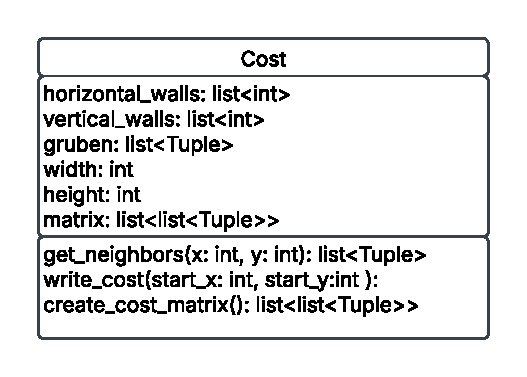
\includegraphics[width=0.6\textwidth]{Simultane Labyrinthe/pdf_src/cost_diagramm.pdf}
  \caption{Cost Klasse}
  \label{fig:cost_diagramm}
\end{figure}
\\
Für jedes Labyrinth wird ein Cost-Objekt erstellt und die Methode $cost_obj.create_cost_matrix()$ aufgerufen. 
Das Cost-Objekt bekommt als Übergabewerte die horizontalen und vertikalten Wände, die  Gruben sowie die Größe des Labyrinths.\\
\begin{lstlisting}[caption={Methode \texttt{create\_cost\_matrix}}, label={lst:create_cost_matrix}]
  def create_cost_matrix(self) -> list:
\end{lstlisting}
Die $create\_cost\_matrix$ Methode erstellt zunächst eine leere Liste mit der Dimension [height][width], die als Kostenmatrix dient.
Dann ruft sie die Methode $write\_cost$ auf, um die Kostenmatrix zu füllen.
\vspace{2em}
\begin{lstlisting}[caption={Methode \texttt{write\_cost}}, label={lst:write_cost}]
  def write_cost(self, start_x: int, start_y: int):
\end{lstlisting}
Zu Beginn der Methode $write\_cost()$ wird die Liste $stack$ initalisiert. Sie speichert alle Felder, die noch besucht werden müssen.
Jeder Eintrag in der Liste besitzt vier Werte: die x-Position, die y-Position, die aktuellen Kosten sowie die entgegengesetzte Richtung, aus welcher das Feld betreten wurde. 
Die Startposition wird als erstes Element hinzugefügt.
Anschließend wird das erste Element der Liste entnommen und in die Kostenmatrix übertragen.
Falls es schon in der Kostenmatrix ist, wird es übersprungen.
Daraufhin werden alle benachbarten Felder mit der Methode $get\_neighbours$ ermittelt und dem $stack$ hinzugefügt.
Dabei werden die Kosten um eins erhöht und die jeweilige Richtung gespeichert.
Das wiederholt sich solange bis der $stack$ leer ist.

\subsubsection{Lösen der Labyrinthe}

Zum Lösen der Labyrinthe wird die Klasse $Solving$ benutzt.
\begin{figure}[H]
  \centering
  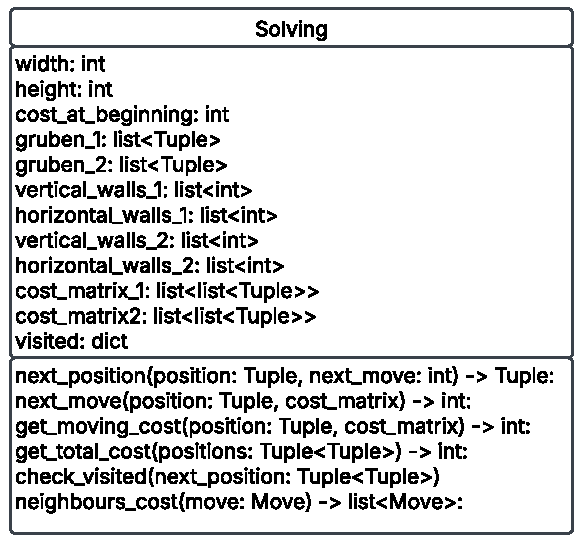
\includegraphics[width=0.6\textwidth]{Simultane Labyrinthe/pdf_src/solving_diagramm.pdf}
  \caption{Solving Klasse}
  \label{fig:solving_diagramm}
\end{figure}
Die Wege werden mit der Klasse $Move$ dargestellt.
\begin{figure}[h]
  \centering
  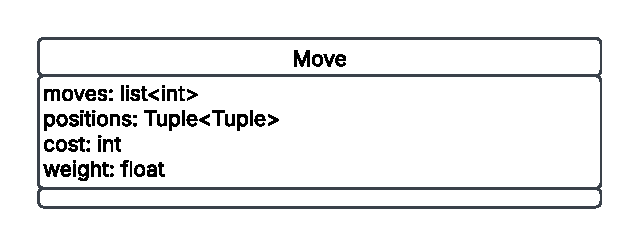
\includegraphics[width=0.6\textwidth]{Simultane Labyrinthe/pdf_src/moving_diagramm.pdf}
  \caption{Move Klasse}
  \label{fig:moving_diagramm}
\end{figure}
\\
Das Attribut $cost$ beschreibt die aufsummierten Kosten der beiden aktuellen Positionen basierend auf den Werten aus den Kostmatrizen.
Das Attribut $weight$ wird gemäß der Gleichung \eqref{weg_kosten} berechnet.\\
\\
Zu Beginn wird ein $Solving$-Objekt initalisiert und eine leere Liste $moves$ angelegt, in der alle aktuellen Wege gespeichert werden.
Anschließend wird ein erstes $Move$-Objekt erzeugt, dessen Startposition ((0, 0), (0, 0)) ist und seine moves leer sind.
In jedem Schritt wird das erste Element aus der $moves$ Liste entnommen.
Dann wird mit folgendem Aufruf
\begin{lstlisting}
  new_moves = solving_obj.neighbours_cost(move)
\end{lstlisting}
\vspace{-2em}
eine Liste von möglichen Folgewege erzeugt.
Die Liste wird mit den neuen Wegen erweitert, sortiert und auf die $l$ besten Wege beschränkt.
\\
\begin{lstlisting}[caption={Methode \texttt{neighbours\_cost}}, label={lst:neighbours_cout}]
  def neighbours_cost(self, move: Move) -> list:
\end{lstlisting}
Zu Beginn der Methode $neighbours\_cost()$ werden die beiden Positionen aus dem Attribut $positions$ des übergebenen $move$-Objekt genommen.
Anschließend werden mit den folgenden Aufrufen
\begin{lstlisting}
  move_1 = self.next_move(pos1, self.cost_matrix_1)
  move_2 = self.next_move(pos2, self.cost_matrix_2)
\end{lstlisting}
\vspace{-2em}
die jeweils nächsten möglichen Richtungen aus der Kostenmatrix bestimmt, falls das Ziel noch nicht erreicht wurde.
Daraufhin werden die neuen zwei Positionspaare berechnet, wenn jeweils in die Richtungen gegangen werden würde.
\begin{lstlisting}
  next_position_1 = self.next_position(move.positions, move_1)
  next_position_2 = self.next_position(move.positions, move_2)
\end{lstlisting}
\vspace{-2em}
Mit dem folgenden Aufruf wird anschließend überprüft, ob die beiden Positionspaare bereits besucht wurden:
\begin{lstlisting}
  move_1 = self.check_visited(next_position_1, len(move.moves) + 1, move_1)
  move_2 = self.check_visited(next_position_2, len(move.moves) + 1, move_2)
\end{lstlisting}
\vspace{-2em}
Zum Schluss wird für jeden möglichen Zug ein $Move$-Objekt erstellt und zusammen in einer Liste übergeben.
Falls einer der neuen Positionspaare bereits besucht wurde oder bereits im Ziel ist, wird der entsprechende Zug nicht übergeben.
\\
\\
Im folgenden ist die Methode $neighbours\_cost$ als Flussdiagramm dargestellt.       
\begin{figure}[H]
  \centering
  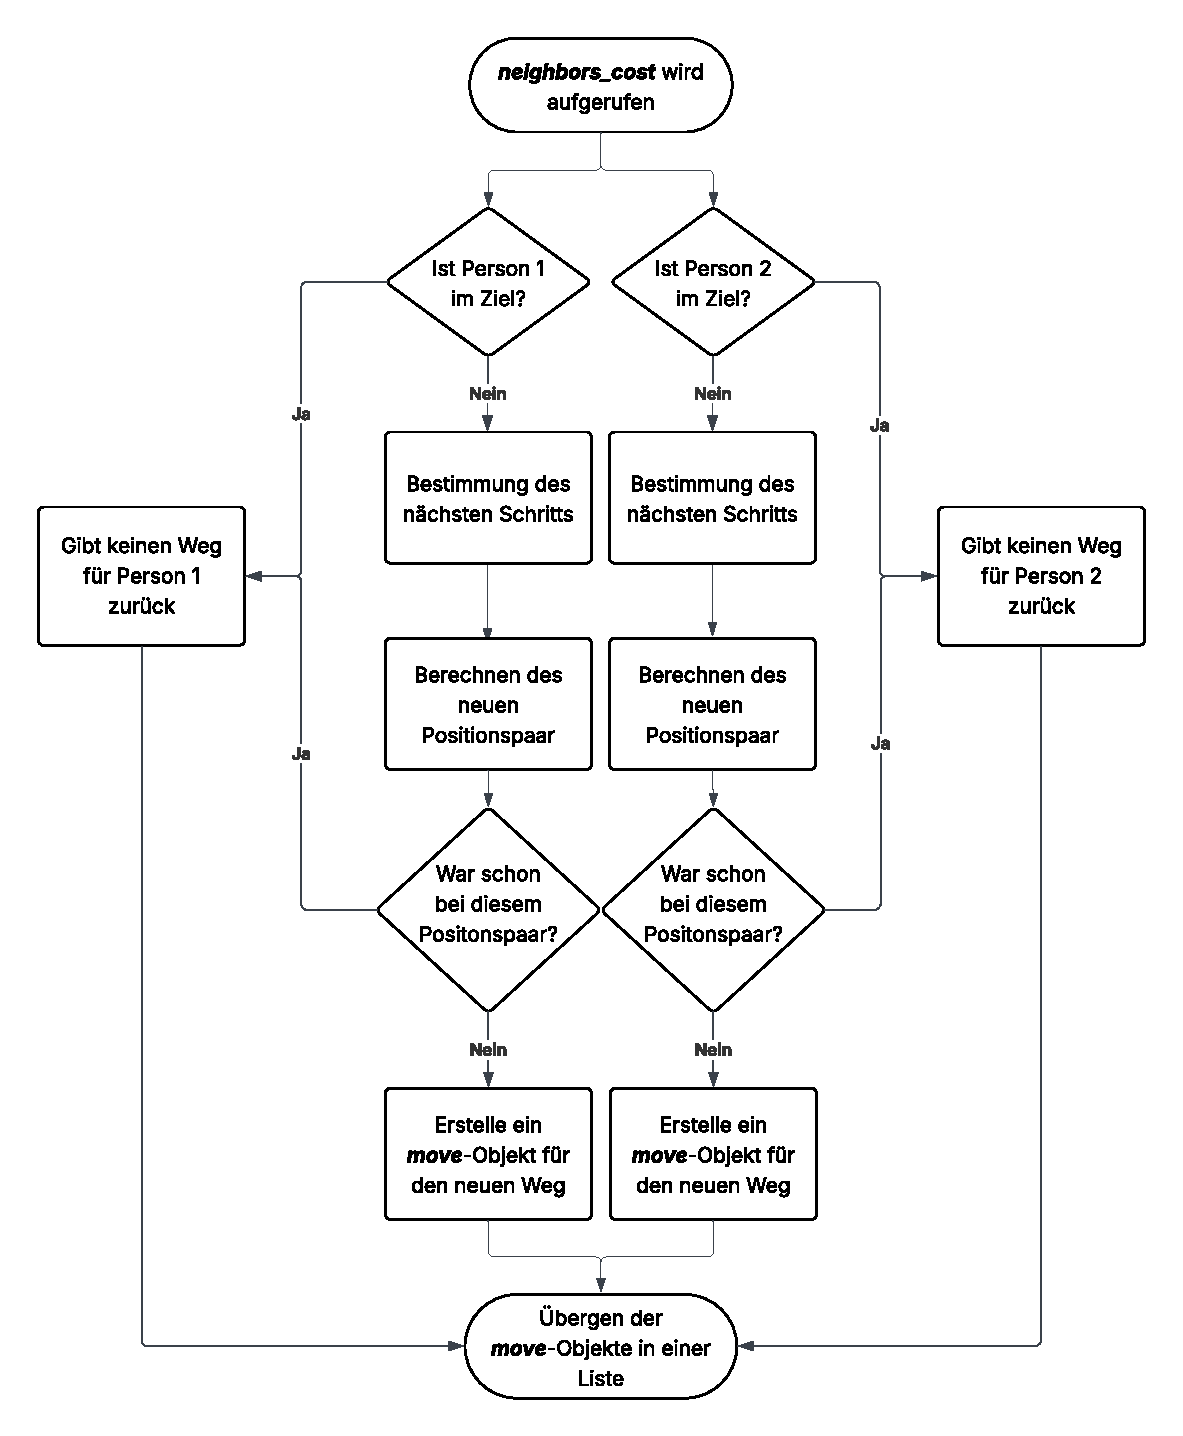
\includegraphics[width=0.8\textwidth]{Simultane Labyrinthe/pdf_src/fluss_diagramm.pdf}
  \caption{$neighbours\_cost$ Flussdiagramm}
  \label{fig:neighbours_cost}
\end{figure}

\subsection{Laufzeit und Diskussion}
\subsubsection{Komplexität der Lösung}
Von jeder Position aus existieren im schlimmsten Fall zwei mögliche Schritte, entweder in Richtung des Ziels von Labyrinth 1 oder in Richtung des Ziels von Labyrinth 2.
Das führt zu insgesammt $2^{\text{maximale Anzahl an Schritten}}$ verschiedenen Möglichkeiten.
Aufgrund dieser großen Anzahl an Möglichkeiten untersucht der Algorithmus nicht alle Pfade vollständig, sondern macht nur eine Abschätzung.
Der hier vorgestellte Ansatz garantiert daher nicht unbedingt den optimalen Lösungsweg, liefert jedoch in akzeptabler Laufzeit eine gute Annäherung.
Der Algorithmus ähnelt einer Tiefensuche, da er einige Wege tief verfolgt, während andere nur kurz betrachtet werden.




\subsubsection{Laufzeit}
Wie schon oben erwähnt beeinflussst die Begrenzung $l$, die Laufzeit und Genauigkeit des Algorithmus stark.
\begin{figure}[h]
  \centering
  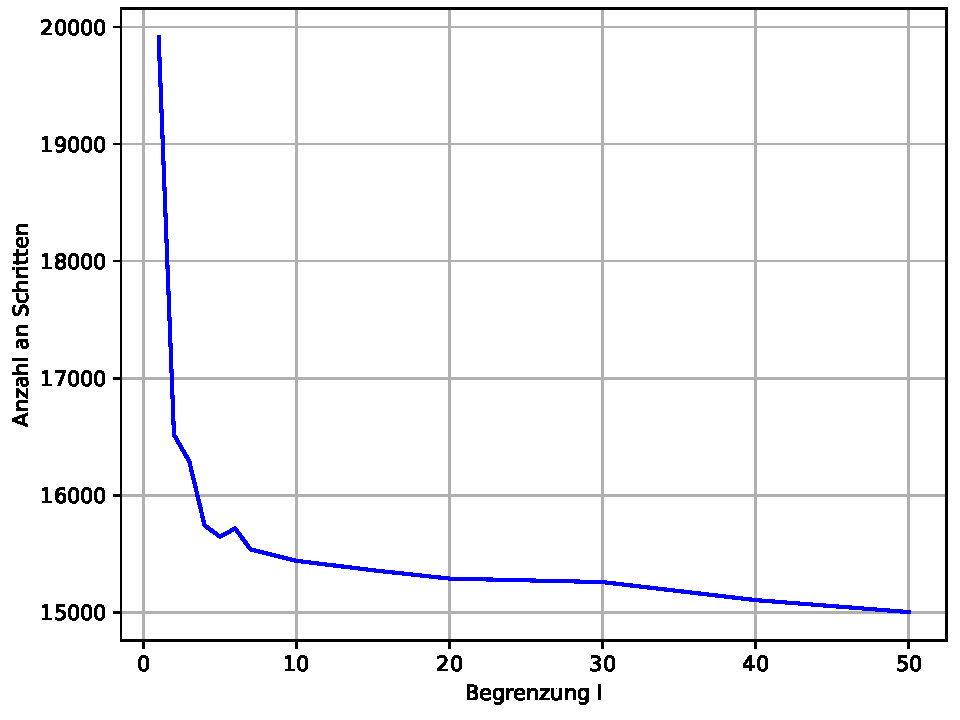
\includegraphics[width=0.5\textwidth]{Simultane Labyrinthe/pdf_src/plotting_schritte_1.pdf}
  \caption{Anzahl der Schritte}
  \label{fig:schritte_1}
\end{figure}
\\
Abbildung \ref{fig:schritte_1} zeigt die Anzahl der Schritte des gefundenen Lösungswegs in Abhängigkeit vom Parameter $l$.
\\
\\
Auffällig ist, dass der Graph mit zunehmendem $l$ gegen die Anzahl der Schritte des optimalen Weges konvergiert.
Ebenso erkennbar ist, dass er nicht streng monoton fallend ist. 
In einem Fall, bei dem die Steigung positiv ist, wird für ein größeren Wert von $l$ ein schlechterer Pfad gefunden.
Dies liegt daran, dass durch den höheren Wert von $l$ neue Wege betrachtet werden.
Diese erscheinen kurzfristig vorteilhafter als die bisherigen Wege und verdrängen dadurch die eigentlich besseren aus der Liste.
Das führt insgesamt zu einem schlechteren Weg.
Bei größeren $l$-Werten tritt dieser Effekt jedoch kaum noch auf, da die Liste groß genug ist, um alle relevanten Pfade zu behalten.
Der Einfluss dieser Monotonieveränderungen wird daher mit wachsendem $l$ vernachlässigbar.

\begin{figure}[H]
  \centering
  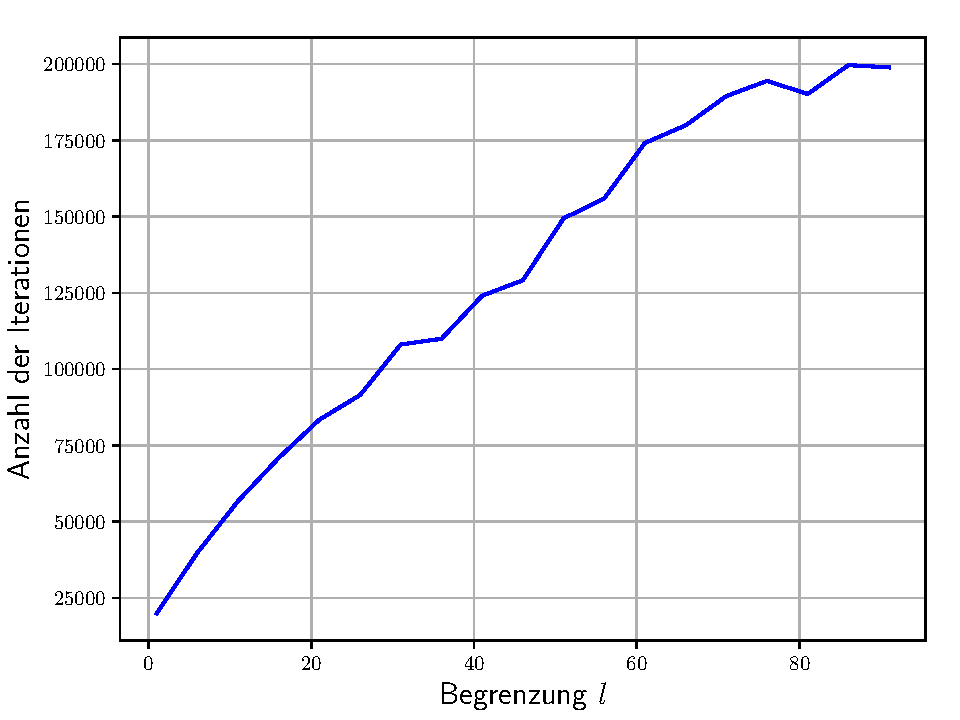
\includegraphics[width=0.5\textwidth]{Simultane Labyrinthe/pdf_src/plotting_laufzeit_1.pdf}
  \caption{maximale Iterationen gegenüber tatsächlichen Iterationen}
  \label{fig:laufzeit_1}
\end{figure}
Abbildung \ref{fig:laufzeit_1} stellt die Anzahl an Iterationen dar, die zur Bestimmung des Lösungswegs benötigt werden in Abhängigkeit vom Parameter $l$.
\\
Der Graph steigt mit wachsendem $l$ stark an.
\\
Allgemein kann die maximale Anzahl an Iterationen in Abhängigkeit von $l$ wie folgt berechnet werden.
\begin{equation}
  l\cdot(2c_1+c_2)
  \label{max_iterationen}
\end{equation}
wobei:\\
- $c_1$ die Kosten vom Startpunkt aus der Kostenmatrix 1 sind\\
- $c_2$ die Kosten vom Startpunkt aus der Kostenmatrix 2 sind\\
Der Faktor $2c_1+c_2$ beschreibt die maximale Anzahl an Schritten, aus denen ein möglicher Lösungsweg bestehen kann.
Zunächst erreicht Agent1 das Ziel mit $c_1$ Schritten.
Anschließend läuft Agent2 denselben Weg zurück in ebenfalls $c_1$ Schritten und geht dann selber ins Ziel mit $c_2$ Schritten.
Im schlechtesten Fall geht er für jeden Eintrag in der Liste, also $l$ mal, die maximale Anzahl an Schritten.
Daher ergibt sich die Gleichung \eqref{max_iterationen}, dies bedeutet, es ergibt sich eine Laufzeit von $o(l)$ ergibt.
Praktisch gesehen ist die Laufzeit aber sehr viel kleiner als die maximale Laufzeit.
\begin{figure}[h]
  \centering
  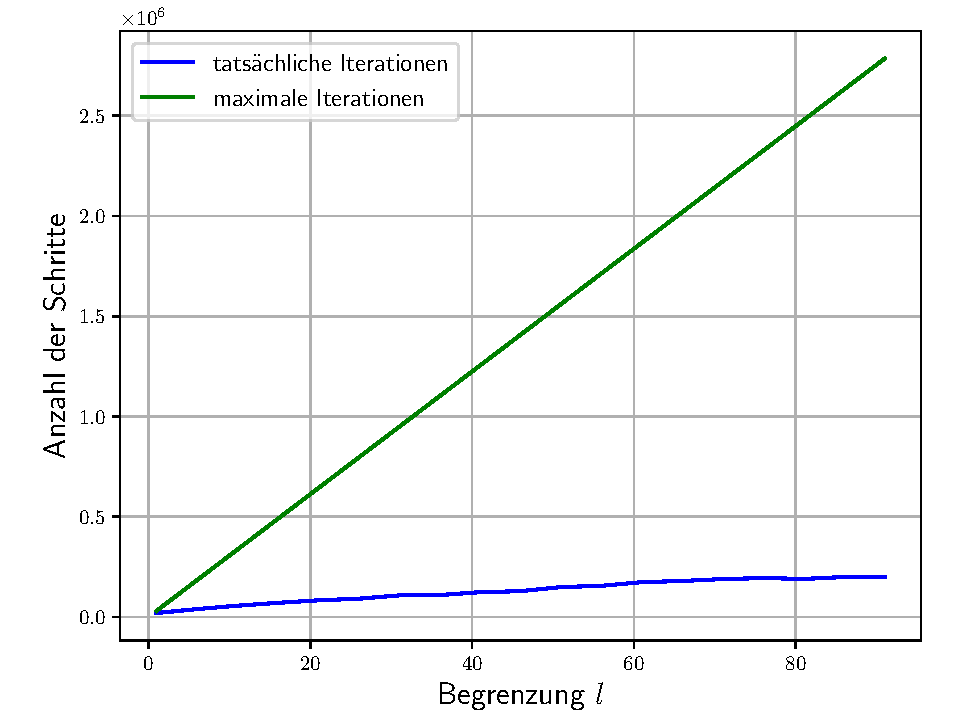
\includegraphics[width=0.5\textwidth]{Simultane Labyrinthe/pdf_src/plotting_max_1.pdf}
  \caption{maximale Iterationen gegenüber tatsächliche Iterationen}
  \label{fig:maximal Laufzeit}
\end{figure}
\\
Der grüne Graph zeigt die maximale Anzahl an Iterationen und der blaue die tatsächliche Anzahl an Iterationen.
\\
\subsubsection{Fazit}
Die Werte von $l$ stehen in einem linearen Zusammenhang mit der Anzahl der Iterationen,
während die Anzahl der Schritte bei größeren $l$-Werten gegen das optimale Ergebnis konvergieren.
Je größer der Wert von $l$, desto mehr Iteration werden durchgeführt - und desto besser wird das Ergebnis.
Die Genauigkeit lässt sich anhand des Parameters $l$ jedoch nicht allgemein bestimmen, da sie stark von der Struktur des jeweiligen Labyrinths abhängt.


\subsection{Vergleich zur Lösung}
Die Musterlösung stellt zwei mögliche Lösungsstrategien vor:\\
1. Breitensuche auf zwei Labyrinthe: Diese Variante wird in der Musterlösung aufgrund ihrer hohe Laufzeit als nicht praktikabel eingestuft.\\
2. A-Star Algorithmus mit Priorty Queue: Diese Option ähnelt stark meiner eigenen Idee. 
Wie in meiner Kostenmatrix wird auch hier für jede Position die Distanz zum Ziel berechnet. 
Unterschied liegt vor allem in einem effizenteren Warteschlagenmodell, das in der Musterlösung verwendet wird.
Insgesamt lagen meine Ergebnisse, aus geschlossen von Testfall 8, bei 1,1\% Abweichung vom optimal Wert. [6]
Bei Testfall 8 fiel mein Ergebnis etwa 3-mal so großes aus, weshalb mir 2 Punke im Kriterium "Verfahren mit guten Ergebnissen" abgezogen wurden.
Außerdem war meine Überlegen zur Laufzeit des Verfahren nicht ausreichend detailiert, was zu einem weiteren Punktabzug führte.\\
Insgesamt erhielt ich für die Aufgabe 17 von 20 Punkten.

\section{Fazit}
-was nehme ich am ende mit\\
-wie gut war ich im Vergleich\\
- was hab ich gelernt\\
- wie gut war das alles jetzt\\

\section{Anhang}
\subsection{Beispiele}
\subsection{Quellcode}
\subsection{Quellen}
[1]  Mordecai J. Golin and Günther Rote,  \textit{A Dynamic Programming Algorithm for Constructing Optimal Prefix-Free Codes with Unequal Letter Costs}, IEEE Transactions on Information Theory 44, no. 5, September 1998

[2] Mordecai J. Golin, Claire Mathieu und Neal E. Young, \textit{HUFFMAN CODING WITH LETTER COSTS: A LINEAR-TIME APPROXIMATION SCHEME}, 2012 Society for Industrial and Applied Mathematics
Vol. 41, No. 3, pp. 684–713

[3] Prof. Justus Piater, \textit{Algorithmen und Datenstrukturen}, 29.05.2024 Universität Innsbruck, Seite 4-13

[4] R. Karp, \textit{Minimum-redundancy coding for the discrete noiseless channel}, IRE Transactions on Information Theory, vol. 7, no. 1, January 1961

[5] \url{https://bwinf.de/fileadmin/wettbewerbe/bundeswettbewerb/43/2_runde/Aufgaben432.pdf}, aufgerufen am 11.10.2025

[6] \url{https://bwinf.de/fileadmin/wettbewerbe/bundeswettbewerb/43/2_runde/Loesungshinweise432.pdf}, aufgerufen am 11.10.2025

[7] \url{https://bwinf.de/bundeswettbewerb/43/}, aufgerufen am 12.10.2025

[8] \url{https://bwinf.de/fileadmin/wettbewerbe/bundeswettbewerb/43/1_runde/431_Statistik.pdf}, aufgerufen am 12.10.2025

[9] \url{https://bwinf.de/fileadmin/wettbewerbe/bundeswettbewerb/43/1_runde/431_Statistik.pdf}, aufgerufen am 12.10.2025

[10] Ralph-Hardo Schulz: \textit{ Codierungstheorie. Eine Einführung. 2. Auflage}, ISBN: 978-3-322-80328-3

\end{document}
